The current trend is to construct programs that play games with imperfect information, for instance Hanabi \cite{DBLP:journals/corr/abs-1902-00506}, but also video games such as Starcraft 2 \cite{DBLP:conf/ijcai/HuLLPX18}. An important ingredient is to reason about higher-order knowledge (an agent knows that another agents knows that...). In these systems, epistemic logic and its dynamic extension, Dynamic epistemic logic (\cite{baltag1998logic}, \cite{DitmarschvdHoekKooi}) may offer formal tools for providing explanations in such AI programs. needs to be understood is relevant in AI, especially in strategic reasoning \cite{DBLP:journals/ijgt/Aumann99}.

The only pedagogical tool we are aware of that explains such models is \emph{Hintikka's world} and was presented at ECAI-IJCAI 2018 \cite{DBLP:conf/ijcai/Schwarzentruber18}. 
\emph{Hintikka's world} is a proof of concept of a graphical user interface that represent Kripke models by  comic strips, as shown in Figure \ref{figure:gui}. It enables to explore mental states of agents. The tool is available at the following address:
\url{http://hintikkasworld.irisa.fr/}. 


Kripke models are graphs, represented explicitly in memory in the first version of the tool. Explicit models are useful to learn how dynamic epistemic logic works by means of toy examples: muddy children, Sally and Anne  \cite{wimmer1983beliefs}, etc.  However, in real card games, such as Hanabi, there are an exponential number of possible configurations of cards. For instance Hanabi has 50 cards total and each player has 4 cards and the order of the cards is important. Therefore with 4 players, the initial Kripke model features $50 \times 49 \times 48 \times \dots \times 38$ configurations, that is $2.2 \times 10^{21}$. Thus, it is impossible to represent explicitly the full graph in memory:  the first version of Hintikka's world does not \emph{scale}. 

That is why, in this demonstration, we propose to represent Kripke models symbolically by using the approach in \cite{DBLP:conf/atal/CharrierS17} and \cite{DBLP:conf/aiml/CharrierS18}. The implementation relies on Binary Decision Diagrams (BDDs) \cite{} as it was done in the tool DEMO\footnote{The current implementation does not rely on DEMO since their work is not well-suited for a web application.}  \cite{DBLP:conf/lori/BenthemEGS15}. 






\begin{figure}
	\begin{center}
		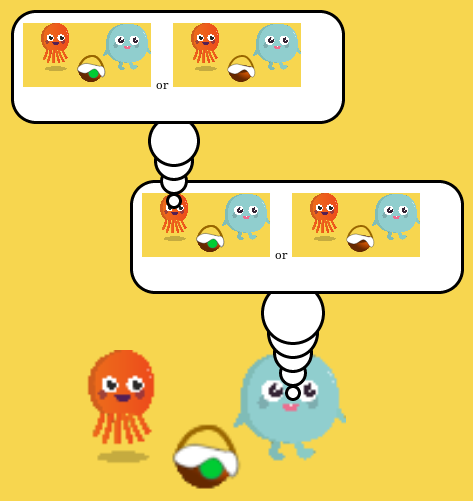
\includegraphics[width=4cm]{screenshot.png} TODO ajouter le modèle de Kripke
	\end{center}
	\caption{Graphical user interface of \emph{Hintikka's world}.\label{figure:gui}}
\end{figure}
